\chapter{Metodologías}
\label{chap:metodologias}

Hubo un tiempo en el que desarrollar un juego no necesitaba mucho más de un equipo pequeño de personas (3 ó 4 como máximo) y no mucho más de 6 meses de esfuerzo \cite{dill-07}, pero la exacerbada competencia que existe actualmente en la industria implica equipos de desarrollo de más de 50 personas expertas trabajando durante varios años con un presupuesto de millones de dólares para lograr publicar un solo videojuego comercial \cite{mor-10}. 

Por tanto, dada la evidente complejidad tanto técnica como personal de un videojuego, es necesario manejar su desarrollo haciendo uso de las metodologías y técnicas de planificación adecuadas que involucren una serie de pasos organizados para guiar cada proceso hasta el resultado final.

En este capítulo se hablará de la metodología de desarrollo de videojuegos más común y a continuación se presenta y justificará la metodología de trabajo seguida a lo largo del desarrollo de \MineRVa.

\section{Metodologías de desarrollo de videojuegos}

Los videojuegos no dejan de ser un recurso informático, aunque están muy próximos en cuanto a consumo y producción al entorno audiovisual. El sistema de producción audiovisual tiene clara relación con gran parte de las fases de desarrollo del videojuego, pero a pesar de ser considerado un software más no existe una metodología común y propia para su diseño y desarrollo \cite{man-14}. El campo del videojuego ya no es sólo una industria que aporta importantes beneficios sino que se convierte en objeto de estudio en lo que a metodologías se refiere \cite{agu-08}.

El desarrollo de un juego, a lo largo de su ciclo de vida, se puede asemejar al de una película de cine, pudiéndose segmentar en tres fases ampliamente diferenciadas: \textbf{pre-producción}, \textbf{producción} y \textbf{post-producción}, cada una con sus etapas características \cite{bet-03}.

\vspace{0.4cm}

\begin{figure}[!h]
    \begin{center}
        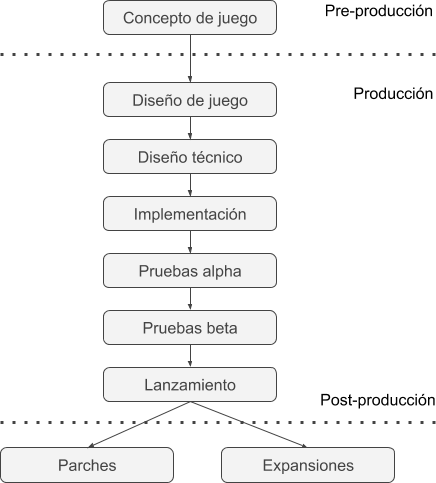
\includegraphics[width=0.625\textwidth]{imagenes/5/pre-prod-post.png}
        \caption{Fases del desarrollo de videojuegos, adaptado de \cite{man-14}}
        \label{fig:fases-desarrollo}
    \end{center}
\end{figure}

Esta metodología puede ser usada con distintos procesos de desarrollo, como \textit{Rational Unified Process}, \textit{Scrum} o \textit{Huddle}. Este último es un proceso especifico de desarrollo de videojuegos y se llama así siguiendo la analogía de Scrum, ya que la reunión que se realiza en el fútbol americano antes de cada jugada se llama \textit{huddle}. Su filosofía es que mediante breves reuniones se planifique cada iteración, permitiendo tanto realizar un seguimiento más específico al avance del proyecto como poder hacer correcciones tempranas ante posibles desviaciones \cite{mor-10}.

Aunque el problema de proyectos privativos como videojuegos a gran escala es que no suele filtrarse mucha información referente a su parte técnica, sí se sabe que uno de los procesos más populares ha sido el de Cascada, aunque poco a poco las compañías han ido migrando a metodologías de desarrollo más flexibles \cite{mor-10}.

A continuación se explican estas fases con más profundidad.

\subsection{Fase de pre-producción}

En la primera fase del proyecto se define el concepto de juego que estamos buscando así como sus aspectos más relevantes, como su \textbf{género}, su \textbf{historia} y sus principales \textbf{bocetos} para obtener una primera idea de su estilo \cite{rou-05}. Además, en esta fase se comienza a dar forma al \acs{GDD}, del que ya se habló en el capítulo \ref{chap:analisis_problema}.

\subsection{Fase de producción}

Esta es la fase más exigente del proyecto. En ella participan multitud de profesionales muy especializados y confluyen toda clase de actividades, como el diseño técnico, el diseño artístico o el diseño mecánico y la implementación y pruebas de los mismos. 

Además, a lo largo de esta fase se generan muchos documentos . Los más importantes son el \acs{GDD}, cuya finalización debería coincidir con la de esta fase, y la \textbf{Biblia del juego}, donde se recogen todas las historias de los personajes, del mundo donde sucede el juego, de su pasado y de los personajes secundarios que aparecen, creando el hilo argumental completo, con todos los detalles \cite{man-14}.

Esta fase termina con la generación del \textbf{gold master}, la copia definitiva que se envía a fábrica para su producción junto con el arte como la portada o el manual de usuario.

\subsection{Fase de post-producción}

Pero como ya sabemos el ciclo de vida de un producto software no termina con su entrega o, en este caso, su lanzamiento al mercado. Además de las tareas de marketing pertinentes, será preciso llevar a cabo un seguimiento adecuado para dar respuesta al comportamiento que el mercado ha tenido en relación al juego, ya que puede llegar a ser muy diferente al esperado.

Las tareas más inmediatas pueden ser parches para arreglar elementos o para ajustar su funcionamiento, y si nuestro juego contempla el lanzamiento de expansiones o DLCs (\textit{downloadable content}) también deberemos hacerlo en esta fase. Además, también deberá realizarse un \textbf{análisis post-portem} del proyecto para saber qué ha ido mal y poder mejorarlo para futuros proyectos.

Como puede verse, el desarrollo de un videojuego es una tarea larga y extremadamente compleja en la que intervienen profesionales de todo tipo y que es orquestada por un equipo de dirección que se encarga de que todo vaya según lo planeado y otro equipo de financiación encargado de que el presupuesto de producción se cumpla \cite{man-14}.

\section{Metodología de trabajo}

A continuación se presenta la metodología de trabajo seguida en el desarrollo de \MineRVa.

Diferencias entre proceso de desarrollo y metodología de desarrollo

\subsection{Proceso de desarrollo}

Agile Software Dev.

Sus 4 principios básicos 

\subsection{Metodología de desarrollo}

Scrum

sus 3 pilares (transparencia, inspecion, adaptacion)

\textcolor{red}{Describirlo? artefactos, eventos, workflow, roles...}